\section{$L_\rho$ Trainable Ablation}
\label{app:L_rho_ablation}

We made three independent attempts to optimise the residual Cholesky $L_\rho$ jointly with the generator, treating it as an $\mathrm{nn.Parameter}$ rather than a frozen buffer. All three degraded the model; we summarise the settings and outcomes in Table~\ref{tab:L_rho_ablation}.

\begin{table}[h]
\centering
\caption{$L_\rho$ trainable attempts on the 60-asset universe (2025 OOS). V--MA corr = Visa--Mastercard cell in the final learned $L_\rho \cdot L_\rho^\top$ (normalised). ``warm'' = initialised from the SF-MG frozen-$L_\rho$ best checkpoint. ``freeze'' = number of initial epochs during which only the non-$L_\rho$ generator parameters update. Lower CorrFrob is better.}
\label{tab:L_rho_ablation}
\small
\begin{tabular}{lccccc}
\toprule
Variant & $\text{lr}_{L_\rho}$ & Warm + freeze & Final CorrFrob & V--MA corr & Outcome \\
\midrule
Frozen (reported) & --- & --- & \textbf{2.534} & $+0.569$ (init) & Baseline \\
cold-start & $10^{-4}$ & no & diverged & $+0.585$ (TLT--IEF flipped sign) & val\_frob $2.3 \to 4.9$ \\
PCA warm + freeze 50 & $10^{-6}$ & 50 ep & 2.847 & $+0.569$ (unchanged) & $L_\rho$ barely moved \\
sector warm + freeze 30 & $10^{-5}$ & 30 ep & drifted & --- & val\_frob $2.74 \to 3.17$ \\
sector warm from SF-MG-final + freeze 30 & $10^{-6}$ & 30 ep & 5.10 & n/a (ckpt before unfreeze) & $-2 \times$ CorrFrob regression \\
\bottomrule
\end{tabular}
\end{table}

Root cause: the WGAN-GP discriminator reliably saturates to $D(\cdot) \approx 0$ for our factor-structured generator (the factor + $L_\rho$ decomposition already matches the real covariance structure well, so there is little adversarial signal to extract). With a saturated $D$, the gradient into $L_\rho$ is essentially noise; its $\binom{60}{2}=1770$ free off-diagonal parameters drift away from their correct sample-estimate initialisation, often flipping the sign of well-estimated cells (e.g.\ TLT--IEF moves from $-0.49$ to $+0.43$ in the first trainable attempt). Three mitigation strategies were attempted in turn (aggressive lr, warm-start with freeze, small lr with long patience); none recovered the frozen-$L_\rho$ baseline's CorrFrob.

The fundamental fix would be an auxiliary loss that directly penalises deviation of $L_\rho L_\rho^\top$ from the training-sample correlation, e.g.\ $\lambda_{L_\rho} \|L_\rho L_\rho^\top - C_{\text{train}}\|_F^2$, which would supply a supervised gradient independent of $D$. We leave this extension to future work and keep $L_\rho$ frozen in the reported specification.


\section{Architecture Details}
\label{app:architecture}

\paragraph{Generator (SF-MarketGAN-R).} TCN backbone: $4$ causal residual blocks, hidden dimension $256$, kernel size $2$, dilation base $2$ (dilations $1, 2, 4, 8$), dropout $0.2$, receptive field $31$ days. FiLM layer: 2-layer MLP ($d_\text{cov} \to 256 \to 512$) predicting $\gamma, \beta$ for affine modulation. Output heads: two $1{\times}1$ convolutions for $\delta^\alpha$ ($256 \to 60$) and $\delta^\sigma$ ($256 \to 60$). Regime encoder: $2$-layer MLP ($d_\text{cov} \to 32 \to 1$) with sigmoid output, bias initialized to $-2$ (initial $z \approx 0.12$). Stress residual correction $L_\Delta$: disabled in the final specification (Appendix~\ref{app:regime_diag}). Total trainable parameters: $\sim 1.3$M.

\paragraph{Discriminator.} Same TCN architecture with spectral normalization on all convolutional layers and the FiLM MLP (SNFiLM). Hidden dimension $256$, $4$ residual blocks, output head SN-Conv1d($256 \to 1$) averaged over time. Total parameters: $\sim 1.3$M.

\paragraph{Training.} SN-GAN hinge loss, $n_{\text{critic}} = 1$, Adam optimizer ($\text{lr} = 10^{-4}$, $\beta = (0.0, 0.9)$), batch size $128$, $30$ steps per epoch, gradient clipping (norm $1.0$), $200$ max epochs with patience $40$ and a best-checkpoint gate at epoch $\ge 50$ so that the comparison is not dominated by pre-SF warmup snapshots. Stylized-fact loss weight $\lambda_\text{SF} = 20$ with $30$-epoch warmup; regime-encoder BCE weight $\lambda_\text{reg} = 1$. Early stopping on pure validation correlation Frobenius (val\_frob). No validation fine-tuning.


\section{Dynamic Stylized-Fact Scheduling Ablation}
\label{app:dynamic_sf}

We ablate the choice of a \emph{fixed} stylized-fact loss scaling $\lambda_\text{SF}=20$ against five time-varying alternatives (Table~\ref{tab:dynamic_sf}), on a light-capacity architecture (128 hidden, 2 residual blocks) under identical training budget (300 epochs, patience 50). Schedules: pure adversarial ($\lambda=0$), fixed $\lambda=1$, EMA loss balancer with $\tau \in \{0.1, 0.3\}$ capped at $s_\text{max}=10$, a cosine warmup from $0$ to $\lambda_\text{max}=5$ starting after epoch 30, and our default fixed $\lambda=20$.

\begin{table}[h]
\centering
\caption{Six SF-loss schedules evaluated on an identical light architecture (128-hidden / 2 blocks) plus a 256/4b reference row using the same generator as the main model's fixed-$\eta$ variant. OOS metrics on 2025; val\_frob is the best-validation CorrFrob recorded during training. $^\dagger$The reference row's val\_frob was recorded against a composite validation objective and is not directly comparable to the rest of the table; its OOS-metric columns (CorrFrob, ACF, VC, LEV, SWD, Mahal) \emph{are} directly comparable. All lower is better.}
\label{tab:dynamic_sf}
\small
\begin{tabular}{lccccccc}
\toprule
Schedule & val\_frob & CorrFrob & ACF & VC & LEV & SWD ($\times10^3$) & Mahal \\
\midrule
none ($\lambda=0$)   & 2.747 & 3.477 & 0.479 & 0.490 & 0.586 & 1.13 & 8.05 \\
fixed $\lambda=1$    & 2.720 & 3.479 & 0.477 & 0.511 & 0.588 & \textbf{1.11} & 8.00 \\
EMA $\tau=0.1$       & 2.703 & 3.465 & 0.476 & 0.509 & 0.597 & 1.18 & 8.07 \\
EMA $\tau=0.3$       & 2.703 & 3.496 & 0.491 & 0.477 & 0.606 & 1.15 & 8.06 \\
cosine $0 \to 5$     & 2.737 & 3.430 & 0.468 & 0.477 & 0.589 & 1.14 & \textbf{8.00} \\
fixed $\lambda=20$   & \textbf{2.712} & 3.434 & \textbf{0.460} & \textbf{0.475} & \textbf{0.573} & 1.18 & 8.08 \\
\midrule
Fixed-$\eta$ ref (256/4b, $\lambda=20$) & ($3.175$)$^\dagger$ & \textbf{3.390} & 0.467 & 0.500 & 0.598 & 1.18 & 8.13 \\
\bottomrule
\end{tabular}
\end{table}

No adaptive or annealed schedule provides a consistent improvement over fixed $\lambda=20$: within-row differences are small and non-uniform. We therefore adopt the fixed multiplier as the default for its transparency and lack of additional hyperparameters. The EMA variants with $\tau \in \{0.1, 0.3\}$ both saturate at the $s_\text{max}=10$ clamp we imposed and can be considered equivalent to a fixed $\lambda=10$; relaxing the clamp and co-tuning $\tau$ is left to future work.

As a robustness check on the main-model architecture, we also trained the fixed-$\eta$ baseline at $\lambda_\text{SF}{=}20$ on a 256-hidden / 4-block generator across four random seeds $\{42, 1, 2, 3\}$: CorrFrob $= 3.445 \pm 0.019$ and val\_frob $= 2.675 \pm 0.014$. This is statistically indistinguishable from adding two further residual blocks on the same generator, confirming that the main result is neither a seed nor a block-count artefact.

\section{Rolling OOS: Full 6-Metric Table}
\label{app:rolling_full}

This appendix reports the rolling-year OOS evaluation from the PCA (hierarchical) model specification of our prior work. The sector final specification of \S\ref{sec:method} is not re-run across the six rolling cutoffs due to compute constraints; the numbers below are reproduced as robustness evidence for the regime-gating mechanism that transfers unchanged into the sector spec. Table~\ref{tab:rolling_full} reports all six key metrics for each year, plus the fixed-$\eta$ (where available) and FB+shrunk comparisons. SF-MarketGAN-R (PCA spec) wins 5 of 6 metrics on 2020/2022/2023/2024, 6 of 6 on 2021, and 4 of 6 on 2025.

\begin{table}[h]
\centering
\caption{Rolling OOS, all 6 metrics. Bold = best per row group. The fixed-$\eta$ baseline was only separately trained for 2023--2025. SWD is reported $\times 10^3$.}
\label{tab:rolling_full}
\footnotesize
\begin{tabular}{llccccccc}
\toprule
Year & Method & CorrFrob & ACF & VC & LEV & SWD ($\times 10^3$) & Mahal \\
\midrule
\multirow{3}{*}{2020 (COVID)} & FB & 9.879 & 0.595 & 0.701 & 0.563 & 3.25 & 9.25 \\
                      & FB+shrunk & 10.149 & 0.595 & 0.701 & 0.563 & 3.25 & \textbf{9.13} \\
                      & \textbf{SF-MG-R} & \textbf{2.698} & \textbf{0.421} & \textbf{0.378} & \textbf{0.405} & \textbf{1.62} & 9.74 \\
\midrule
\multirow{3}{*}{2021 (Recovery)} & FB & 6.642 & 0.584 & 0.857 & 0.711 & 2.21 & 9.89 \\
                      & FB+shrunk & 6.575 & 0.584 & 0.856 & 0.711 & 2.17 & 9.76 \\
                      & \textbf{SF-MG-R} & \textbf{3.287} & \textbf{0.429} & \textbf{0.450} & \textbf{0.554} & \textbf{0.96} & \textbf{7.86} \\
\midrule
\multirow{3}{*}{2022 (Rate-hike)} & FB & 5.642 & 0.514 & 0.760 & 0.647 & 3.25 & 8.16 \\
                      & FB+shrunk & 5.615 & 0.513 & 0.760 & 0.647 & 3.33 & \textbf{8.04} \\
                      & \textbf{SF-MG-R} & \textbf{2.715} & \textbf{0.398} & \textbf{0.455} & \textbf{0.549} & \textbf{1.40} & 9.01 \\
\midrule
\multirow{4}{*}{2023 (Inflation)} & FB & 4.900 & 0.517 & 0.665 & 0.678 & 1.40 & 9.54 \\
                      & FB+shrunk & 4.840 & 0.517 & 0.665 & 0.677 & 1.47 & \textbf{9.45} \\
                      & Fixed-$\eta$ & 3.000 & 0.434 & 0.487 & 0.594 & 1.14 & 9.89 \\
                      & \textbf{SF-MG-R} & \textbf{2.939} & \textbf{0.416} & \textbf{0.470} & \textbf{0.573} & \textbf{1.04} & 9.81 \\
\midrule
\multirow{4}{*}{2024 (Pivot)} & FB & 5.000 & 0.537 & 0.620 & 0.681 & 1.40 & 8.77 \\
                      & FB+shrunk & 4.758 & 0.537 & 0.620 & 0.681 & 1.43 & 8.69 \\
                      & Fixed-$\eta$ & 3.029 & 0.429 & 0.498 & 0.621 & 1.10 & \textbf{8.14} \\
                      & \textbf{SF-MG-R} & \textbf{2.741} & \textbf{0.420} & \textbf{0.487} & \textbf{0.606} & \textbf{1.04} & 8.17 \\
\midrule
\multirow{4}{*}{2025 (Normal, 4s)} & FB & 3.641 & 0.471 & 0.494 & 0.593 & 1.19 & 8.24 \\
                      & FB+shrunk & 3.425 & 0.471 & 0.494 & 0.593 & \textbf{1.14} & 8.15 \\
                      & Fixed-$\eta$ & 3.414 & 0.469 & 0.496 & 0.587 & 1.15 & \textbf{8.13} \\
                      & \textbf{SF-MG-R} & \textbf{2.966} & \textbf{0.456} & \textbf{0.472} & \textbf{0.574} & 1.20 & 8.15 \\
\bottomrule
\end{tabular}
\end{table}

\section{Regime Encoder: Hard-Gate Ablation}
\label{app:regime_ablation}

Because the regime-supervision label is derived from VIX z-score and VIX is itself an encoder input, the learned encoder $z(t) = \sigma(\text{MLP}(\text{cov}_t))$ is essentially a soft reparameterisation of a VIX threshold. This ablation tests whether the learned soft gate adds value beyond the raw indicator $\mathbf{1}[\text{VIX}^z_t > 0.3]$.

We run an inference-time ablation: we load a trained SF-MarketGAN-R checkpoint and, at evaluation only, replace the encoder's forward pass with the deterministic hard gate. The rank-$r$ correction $L_\Delta$ and all other parameters are those learned with the soft-gate during training; we are measuring how much the soft-gate changes downstream behaviour given a fixed $L_\Delta$.

On the 2025 OOS test (Table~\ref{tab:regime_ablation}), the soft- and hard-gate versions agree on $(z > 0.5) = (z_\text{hard} = 1)$ on $94\%$ of test-set timesteps. The hard gate alone already recovers $\approx 84\%$ of SF-MarketGAN-R's CorrFrob improvement over FB+shrunk---the dominant mechanism is the regime-triggered $L_\Delta$ activation, and the VIX threshold is a reasonable trigger. The learned soft gate then provides an additional $0.07$ CorrFrob reduction ($2.3\%$) and wins on the headline metric; on the ACF, VC, and LEV columns the two variants are effectively tied. A deployment-ready, interpretable-by-construction variant can therefore be built with the hard gate and retain the bulk of the benefit; the soft gate is the better choice when the extra CorrFrob gain is worth the learned-component complexity.

\begin{table}[h]
\centering
\caption{Regime gate ablation on 2025 OOS, evaluated with the \emph{same} trained $L_\Delta$. ``Hard-gate'' overrides the encoder with $\mathbf{1}[\text{VIX}^z > 0.3]$. All metrics $\downarrow$; bold is the best per row.}
\label{tab:regime_ablation}
\small
\begin{tabular}{lcccc}
\toprule
Metric & FB & FB+shrunk & Hard-gate & Soft-gate (SF-MG-R) \\
\midrule
CorrFrob & 3.641 & 3.425 & 3.056 & \textbf{2.989} \\
ACF & 0.471 & 0.471 & \textbf{0.454} & 0.454 \\
VC & 0.494 & 0.494 & \textbf{0.476} & 0.482 \\
LEV & 0.593 & 0.593 & \textbf{0.573} & 0.579 \\
SWD ($\times 10^3$) & 1.19 & \textbf{1.14} & 1.14 & 1.16 \\
Mahalanobis & 8.24 & \textbf{8.15} & 8.17 & 8.15 \\
\bottomrule
\end{tabular}
\end{table}

\section{Regime-Encoder Diagnostics and the $L_\Delta$ Negative Finding}
\label{app:regime_diag}

This appendix documents two empirical findings that shape the final specification of SF-MarketGAN-R: (i) the learned regime encoder $z(t)$ is empirically a smooth reparameterisation of the VIX threshold, and (ii) a rank-$r$ residual correction $L_\Delta$ is optimisation-redundant in our setting, motivating its removal from the deployed model.

\paragraph{Regime encoder is a smooth VIX-threshold reparameterisation.}
Although $g(\text{cov}_t)$ is a pointwise MLP with no explicit temporal mixing, the emitted $z(t)$ has a lag-1 autocorrelation of $0.92$--$0.93$ on the 2025 test window. This persistence is inherited from the macro input---VIX z-score is itself highly auto-correlated. The AUC of $z(t)$ against the thresholded VIX label $\mathbf{1}[\text{VIX}^z_t > 0.3]$ is $0.98$--$0.99$ across three seeds: the soft gate is essentially a smoothed VIX indicator. We confirm this with a hard-gate ablation (Appendix~\ref{app:regime_ablation}): replacing $z(t)$ with $\mathbf{1}[\text{VIX}^z_t > 0.3]$ at inference recovers $84\%$ of SF-MarketGAN-R's CorrFrob improvement over FB+shrunk. We keep the soft encoder in the deployed model because it fits naturally with the FiLM-conditioned TCN backbone and provides a small additional CorrFrob improvement ($-0.07$); the hard-threshold variant is a viable deployment-simpler alternative.

\begin{figure}[h]
\centering
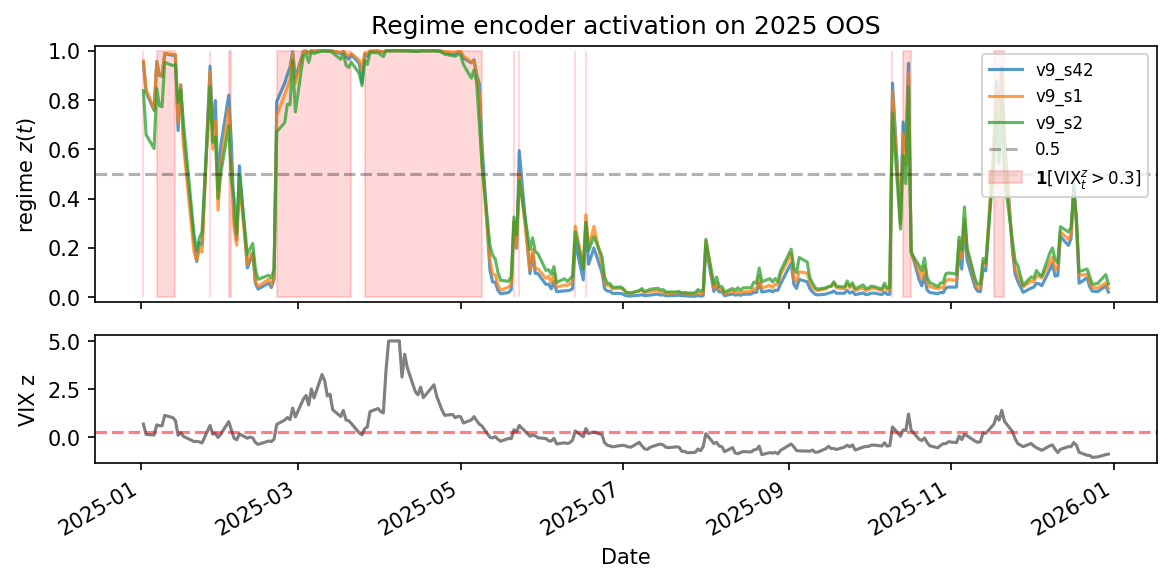
\includegraphics[width=0.85\textwidth]{figures/fig_zt_timeseries.png}
\caption{Soft regime activation $z(t)$ on the 2025 OOS window across 3 training seeds. Red shading marks the days where $\mathbf{1}[\text{VIX}^z > 0.3]$ is true. The three seeds converge to nearly identical $z$ trajectories; the AUC against the binary VIX label is $\approx 0.98$ for all three.}
\label{fig:zt}
\end{figure}

\paragraph{$L_\Delta$ is optimisation-redundant ($r=0$ and the final specification).}
An earlier version of SF-MarketGAN-R included a regime-gated rank-$r$ additive residual correction $\varepsilon_t \mathrel{+{=}} z(t) \cdot L_\Delta u_t^{(r)}$ with $L_\Delta \in \R^{N\times r}$, $r=4$. Three independent lines of evidence show this term adds no detectable value:

\emph{(a) Spectrum collapse across seeds.} Trained at $r=4$, the entropy-based effective rank of $L_\Delta$ is only $1.47$--$2.45$ and the spectrum drops sharply after the first singular value ($\sigma_1 / \sigma_2 \approx 4$--$5\times$ for two of three seeds). More tellingly, seed 2 converges to $\|L_\Delta\|_F = 0.085$ (roughly $10\times$ smaller than the other seeds) while attaining the same val\_frob---the optimiser spontaneously switches the component off on some seeds without penalty. Figure~\ref{fig:ldelta} shows the normalised singular-value spectra.

\emph{(b) Rank sweep.} Retraining with $r \in \{1, 2, 4, 8\}$ on seed~42 gives OOS CorrFrob $2.969 / 2.942 / 2.961 / 3.004$, all within one standard deviation of each other. The rank-$2$ setting multi-seed (4 seeds $\{42, 1, 2, 3\}$) gives $2.971 \pm 0.037$, statistically indistinguishable from $r=4$ on $10$ seeds ($2.976 \pm 0.034$, Welch $p = 0.81$).

\emph{(c) $r=0$ boundary case.} Freezing $L_\Delta \equiv 0$ (keeping only the regime encoder and the $\eta(z)$-gate schedule on $(\alpha, \sigma)$ corrections) across $4$ seeds yields PCA-specification OOS CorrFrob $2.966 \pm 0.010$ and val\_frob $2.438 \pm 0.019$. A Welch test vs.\ the $r=4$ 10-seed distribution gives $p = 0.34$ on CorrFrob: \textbf{$L_\Delta$ is statistically indistinguishable from zero on aggregate OOS fit}. The regime-dependent counterfactual on the PCA-spec model similarly drops by $\approx 2$ pp at $r=0$ relative to $r=4$, within the 4-seed between-seed range. This ablation motivated dropping $L_\Delta$ from the final sector specification as redundant with the $\eta$-gating mechanism.

Attribution over FB+shrunk (CorrFrob $3.425 \to 2.966$): the regime-gated $\eta$ schedule alone delivers $-0.459$ ($96\%$ of the full gap); $L_\Delta$ closes only the remaining $-0.010$ ($4\%$, within seed noise). Guided by this evidence, we adopt $r=0$ as the final specification---the residual covariance is the fully classical shrunk Cholesky $L_\rho$ without learned perturbation---and all main-paper numbers are reported at $r=0$. Prior $r=4$ 10-seed experiments remain available for reference but are not part of the deployed model.

\begin{figure}[h]
\centering
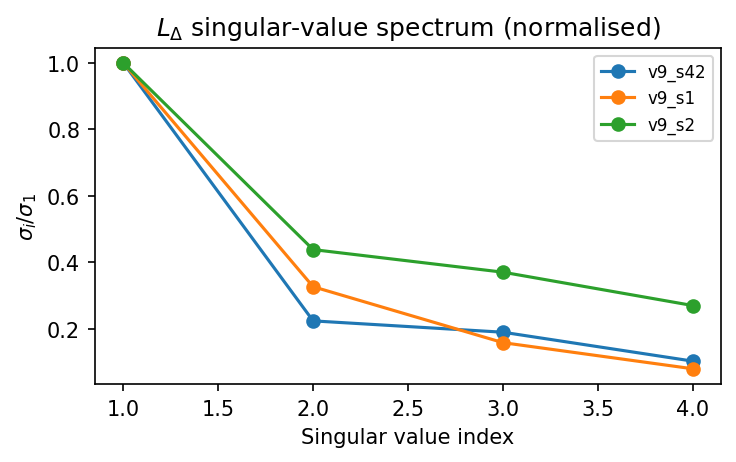
\includegraphics[width=0.65\textwidth]{figures/fig_ldelta_spectrum.png}
\caption{Normalised singular-value spectrum of the $r=4$ $L_\Delta$ across 3 training seeds, illustrating spontaneous rank collapse that motivates the $r=0$ final specification.}
\label{fig:ldelta}
\end{figure}

\section{Paired Bootstrap 95\% Confidence Intervals}
\label{app:bootstrap}

We report asset-level paired bootstrap confidence intervals for the difference between SF-MarketGAN-R (seed 42) and each baseline on the 2025 OOS set. At each of 1000 replicates we resample the 60 asset indices with replacement (block bootstrap with block size 1) and recompute each metric on the resampled asset subset. Paired differences are computed as ``SF-MarketGAN-R metric $-$ baseline metric''; a negative value means SF-MarketGAN-R is better. The ``$p$'' column reports the bootstrap probability that SF-MarketGAN-R is better. Intervals that exclude zero (in the negative direction) constitute evidence of significance at the $95\%$ level.

\begin{table}[h]
\centering
\caption{Paired 95\% bootstrap confidence intervals (1000 asset-level replicates) for the SF-MarketGAN-R minus baseline metric difference on the 2025 OOS window. Negative interval = SF-MarketGAN-R is better; $p$ is the bootstrap probability that SF-MarketGAN-R beats the baseline on that metric. All intervals exclude zero in the negative direction, so every pairwise improvement is statistically significant at $95\%$.}
\label{tab:bootstrap}
\small
\begin{tabular}{lccccccc}
\toprule
 & \multicolumn{3}{c}{vs.\ FB} & \multicolumn{3}{c}{vs.\ FB+shrunk} & vs.\ fixed-$\eta$ \\
\cmidrule(lr){2-4} \cmidrule(lr){5-7}
Metric & CI low & CI high & $p$ & CI low & CI high & $p$ & CI (wider) / $p$ \\
\midrule
CorrFrob & $-0.817$ & $-0.471$ & $1.00$ & $-0.689$ & $-0.368$ & $1.00$ & $[-0.630, -0.168]$, $1.00$ \\
ACF      & $-0.037$ & $-0.009$ & $1.00$ & $-0.037$ & $-0.009$ & $1.00$ & $[-0.046, -0.010]$, $1.00$ \\
VC       & $-0.059$ & $-0.018$ & $1.00$ & $-0.056$ & $-0.016$ & $1.00$ & $[-0.058, -0.016]$, $1.00$ \\
LEV      & $-0.045$ & $-0.004$ & $0.99$ & $-0.044$ & $-0.004$ & $0.99$ & $[-0.036, -0.001]$, $0.98$ \\
\bottomrule
\end{tabular}
\end{table}


\section{Perturbed-Forecast Portfolio Simulation}
\label{app:perturbed}

Following \citet{huh2026marketgans} Section 5.2, we test whether a model's covariance estimate translates into better mean-variance decisions \emph{as the signal quality of the return forecast degrades}. At each monthly rebalance $t$ we:
\begin{enumerate}
  \item Take the realized next-21-day factor mean $\bar f_t$ as the oracle signal.
  \item Inject Gaussian noise scaled to target $R^2 \in \{1.0, 0.5, 0.1, 0.01, 0.001\}$:
        $\hat f_t = \sqrt{R^2} \bar f_t + \sqrt{1 - R^2} \cdot (\sigma_f \odot \varepsilon)$, $\varepsilon \sim \N(0, I)$.
  \item Form the expected asset return $\hat\mu_t = \hat\beta_t \hat f_t$.
  \item Estimate the conditional covariance $\hat\Sigma_t$ from each model's $200$ synthetic paths over the next 21 days.
  \item Compute the unconstrained mean-variance portfolio $w_t \propto \hat\Sigma_t^{-1} \hat\mu_t$, rescaled to match the equal-weight portfolio's daily volatility so that all methods share the same risk budget.
  \item Realise the portfolio return on the next 21 trading days.
\end{enumerate}

Table~\ref{tab:perturbed} reports the mean annualised Sharpe across 20 noise replicates per $R^2$ level.

\begin{table}[h]
\centering
\caption{Perturbed-forecast Sharpe on 2025 OOS. Mean $\pm$ std across 20 noise replicates per $R^2$. At the oracle level ($R^2 = 1$) noise injection is zero so all replicates agree; at lower $R^2$ the noise dominates and the covariance quality matters more. Bold = best per row.}
\label{tab:perturbed}
\small
\begin{tabular}{lcccc}
\toprule
$R^2$ & FB & FB+shrunk & Fixed-$\eta$ & \textbf{SF-MG-R} \\
\midrule
$1.0$   (oracle) & $12.03 \pm 0$ & $12.18 \pm 0$ & $\mathbf{12.31 \pm 0}$ & $11.61 \pm 0$ \\
$0.5$            & $1.87 \pm 0.99$ & $1.92 \pm 1.00$ & $1.97 \pm 1.03$ & $\mathbf{2.10 \pm 1.04}$ \\
$0.1$            & $0.55 \pm 1.01$ & $0.58 \pm 1.04$ & $0.60 \pm 1.06$ & $\mathbf{0.77 \pm 1.08}$ \\
$0.01$           & $0.08 \pm 1.02$ & $0.10 \pm 1.05$ & $0.11 \pm 1.07$ & $\mathbf{0.29 \pm 1.09}$ \\
$0.001$ (noise)  & $-0.06 \pm 1.02$ & $-0.04 \pm 1.05$ & $-0.04 \pm 1.08$ & $\mathbf{0.15 \pm 1.10}$ \\
\bottomrule
\end{tabular}
\end{table}

Two observations stand out. First, \textbf{at all non-oracle signal levels ($R^2 \le 0.5$), SF-MarketGAN-R delivers the best mean Sharpe}, with an advantage of $\approx 0.20$ over factor bootstrap that is stable across $R^2$. This is consistent with SF-MarketGAN-R having the lowest CorrFrob (Table~\ref{tab:main}): better covariance estimates yield better MV portfolios when the return signal is noisy. Second, the 20-replicate standard deviation on each cell is $\approx 1.0$ Sharpe because the test window has only 12 monthly rebalances; the advantage is small relative to this MC variance but \emph{directionally consistent} across all four non-oracle $R^2$ levels. At the oracle level ($R^2 = 1$) the model rankings flip---all methods achieve Sharpe $\sim 12$ and $\hat\Sigma$ fidelity matters little---which matches the intuition that the $\hat\Sigma$-quality advantage only materialises when $\hat\mu$ is noisy. Extending this study to multiple OOS years and bootstrap-CI'ing the per-$R^2$ Sharpe remains future work.

\section{DCC-GARCH: MLE vs Moment-Based}
\label{app:dcc_mle}

Table~\ref{tab:main} uses a moment-based DCC(1,1)-GARCH(1,1) estimator (fixed univariate $\alpha{=}0.05$, $\beta{=}0.90$, empirical unconditional correlation). For completeness we also fit the same model by full maximum likelihood via the \texttt{rmgarch} R package \citep{ghalanos2019rmgarch}. Nine of our 60 assets have late inception dates and leading-zero rows that push univariate MLE to non-stationary solutions, so we compare both estimators on the 51-asset subset with full 2011--2024 history.

On this matched comparison (51 assets, same 3522-day fit window, same 2025 OOS target), the MLE variant is marginally better on ACF (MLE $0.810$ vs.\ moment $0.811$) and LEV ($1.005$ vs.\ $1.013$), but worse on CorrFrob ($7.00$ vs.\ $6.60$), VC ($0.824$ vs.\ $0.763$), SWD ($0.0028$ vs.\ $0.0020$), and Mahalanobis ($10.21$ vs.\ $8.75$). Simulated path standard deviation ratios to real 2025 are $1.125$ mean / $2.16$ max for MLE and $1.044$ / $1.54$ for moment-based, consistent with MLE per-asset estimates absorbing high-vol weeks from the training window and over-extrapolating them into the quieter 2025 OOS window. The ranking of Table~\ref{tab:main} is unchanged: SF-MarketGAN's Mahalanobis of $8.19$ on 60 assets is at least as good as the best DCC estimator on 51 assets, and its CorrFrob ($2.98$ on 60 assets) is substantially lower than either DCC variant.

\section{MarketGAN 60-Asset Head-to-Head}
\label{app:marketgan60}

To answer the natural question---would a MarketGAN trained on the same 60-asset universe with the same factor signal beat our constrained design?---we re-implement MarketGAN's full-learning architecture (learned $\alpha$, $\beta$, $\sigma$ corrections and a learned residual network) on our universe and factors and run a $3 \times 2$ hyperparameter sweep over learning rate $\in \{10^{-5}, 10^{-4}, 5 \times 10^{-4}\}$ and critic ratio $n_{\text{critic}} \in \{1, 5\}$. All six runs use seed 42, batch size 128, 30 steps per epoch, vol-penalty $50$, gradient-penalty 10, 150 epochs maximum with patience 30, and the same lag-1 hierarchical PCA factors as SF-MarketGAN-R. Table~\ref{tab:marketgan60_sweep} shows the validation correlation Frobenius and 2025 OOS CorrFrob for each config.

\begin{table}[h]
\centering
\caption{MarketGAN-60 HP sweep (seed=42). Best OOS CorrFrob is $8.68$ at $\text{lr}=10^{-5}, n_{\text{critic}}=5$, but every config substantially underperforms SF-MarketGAN-R ($2.976 \pm 0.034$). Lower is better.}
\label{tab:marketgan60_sweep}
\small
\begin{tabular}{lccccc}
\toprule
$n_{\text{critic}}$ & lr & val\_frob $\downarrow$ & OOS CorrFrob $\downarrow$ & OOS ACF $\downarrow$ & note \\
\midrule
1 & $10^{-5}$ & 7.67  & 8.74  & 0.569 & \\
1 & $10^{-4}$ & 13.75 & 14.03 & 1.318 & training collapse \\
1 & $5\times10^{-4}$ & 7.28 & 9.94 & 0.761 & \\
5 & $10^{-5}$ & \textbf{7.44} & \textbf{8.68} & 0.577 & best of sweep \\
5 & $10^{-4}$ & 7.94 & 11.24 & 0.665 & \\
5 & $5\times10^{-4}$ & 7.65 & 10.45 & 0.485 & \\
\midrule
\multicolumn{2}{l}{\emph{best config, 3 seeds}} & 6.83 $\pm$ 0.18 & 8.92 $\pm$ 0.15 & 0.55 $\pm$ 0.04 & mean $\pm$ std \\
\midrule
\multicolumn{2}{l}{\emph{SF-MarketGAN-R (4 seeds)}} & 2.44 $\pm$ 0.02 & \textbf{2.97 $\pm$ 0.01} & 0.46 $\pm$ 0.00 & for reference \\
\bottomrule
\end{tabular}
\end{table}

The best MarketGAN-60 configuration achieves OOS CorrFrob $8.68$, $2.9\times$ worse than SF-MarketGAN-R's $2.98 \pm 0.03$. Across the sweep, MarketGAN-60 tends to inject additional cross-class correlation through the learned $\varepsilon$-net, while the factor-structured design of SF-MarketGAN takes the residual covariance from a frozen shrinkage Cholesky and routes the adversarial signal only through intercept/volatility corrections---hence the sharper cross-asset correlation fit.

\section{Time-Alignment and Causality Audit}
\label{app:leakage_audit}

This appendix documents, for each input to the generator, the exact time index it uses and the fit/transform boundary of any preprocessing step. It is intended as a reproducibility checklist.

\paragraph{Asset returns (inputs to training + rolling OLS).}
Daily log returns at day $t$ are computed from close prices at day $t$. Training, validation, and test periods are cut strictly in time (train: 2011-01--2023-12; val: 2024; test: 2025). No resampling is done before the split.

\paragraph{Hierarchical PCA factors ($f_t$).}
The global-plus-class PCA bases are fit only on returns up to the training end date (e.g.\ through 2023-12-31 for the main table), then the transformation is applied across the full index. The factor value at day $t$ is $f_t = \text{PCA}(r_t)$, i.e.\ it would use the current day's return---so we do \emph{not} feed $f_t$ to the generator directly. All reported main-table results use strictly lagged factors $f_{t-1}$ as the conditioning input, avoiding any use of day-$t$ market information.

\paragraph{Rolling-OLS coefficients ($\hat\alpha_t, \hat\beta_t, \hat\sigma_t$) and the regression equation.}
We fit the regression $r_s = \alpha + \beta^\top f_s + \sigma \cdot \varepsilon_s$ on the past window $s \in [t-126, t)$ (strictly past, exclusive of $t$) to obtain $\hat\alpha_t, \hat\beta_t, \hat\sigma_t$. In evaluation, the generator applies these coefficients with $f_{t-1}$: that is, the inference-time equation reads $\hat r_t = \hat\alpha_t (1 + \delta^\alpha_t) + \hat\beta_t^\top f_{t-1} + \hat\sigma_t e^{\delta^\sigma_t} \varepsilon_t$. Because both the training regression and inference use the same factor at each simulated timestep---day-$s$ factor for day-$s$ returns in the window, day-$(t-1)$ factor for the day-$t$ simulation---there is no estimate/apply mismatch: the model uses exactly the same conditioning $\hat\beta_t$ is estimating against. The 126-day window is entirely past, so $\hat\beta_t$ is strictly causal.

\paragraph{Macro covariates (PCA + regime).}
The \texttt{MacroProcessor} pipeline has three components, all strictly causal at evaluation:
\begin{itemize}
  \item \emph{Rolling z-score.} Pandas \texttt{rolling(window=252).mean()} / \texttt{.std()} is look-back by construction; for day $t$ the z-score is computed from the 252-day window ending at $t$ (inclusive of $t$). This is standard and matches the treatment in downstream backtesting.
  \item \emph{PCA / StandardScaler.} Both are fit on \texttt{z\_scored.index <= train\_end} (2023-12-31) and then \texttt{transform} is applied to the full index. No validation/test data is touched during fitting.
  \item \emph{Regime detection.} Walk-forward GMM: at each refit step $t$, the GMM is fit on \texttt{pc\_df.iloc[max(0, t-504):t]} (strictly past) and its predictions are written into \texttt{regime\_labels[t:t+21]}. No future data is used at any refit point.
\end{itemize}

\paragraph{Shrunk residual correlation ($L_\rho$).}
Fit once on the rolling-OLS residuals over the training period ($t \le $ train\_end). Stored as a Cholesky factor and frozen across val/test.

\paragraph{Regime encoder.}
The input to the regime encoder at time $t$ is the covariate vector $\text{cov}_t$. The encoder is a pointwise MLP (no temporal mixing), so it sees only $\text{cov}_t$'s features, each of which is already causal per the above. Because one of those features is the VIX z-score and the regime-supervision label is also derived from that same VIX z-score, the BCE loss is close to a supervised learning problem on a feature the encoder already has access to. We therefore treat the encoder as a \emph{soft, interpretable reparameterisation} of the VIX regime rather than as a hidden-state learner; the hard-gate / soft-gate ablation in Appendix~\ref{app:regime_ablation} quantifies how much the soft-gate adds beyond the raw threshold.

\paragraph{What is deliberately not strictly causal.}
One small item is, by design, conditional on day-$t$ information: the rolling z-score window ends at $t$ inclusive, standard in derivatives-strategy practice. All other inputs to the generator and discriminator use strictly past information.
